% !TeX spellcheck = en_US
\documentclass[letterpaper,12pt,twoside]{report}
\usepackage{fancyhdr}
\usepackage{fullpage}
\usepackage{tikz}
\usepackage{amsmath}
\usepackage{textcomp}

\begin{document}
	\pagestyle{fancy}
	\fancyhf{}
	\fancyhead[L]{Day 6}
	\fancyhead[R]{\textit{The Calendar Project}}
	\fancyfoot[L]{Citations Involved: none}
	
	% Problem
	\paragraph{Problem}
	\begin{quote}
	\textsf{An equilateral triangle is inscribed in a circle of radius 6 in. A second equilateral triangle is circumscribed about the circle. If the sides of the triangles are parallel, what is the shortest distance from a point on one triangle to a point on the other?}
	\end{quote}
	
	% Graphics
	\begin{center}
		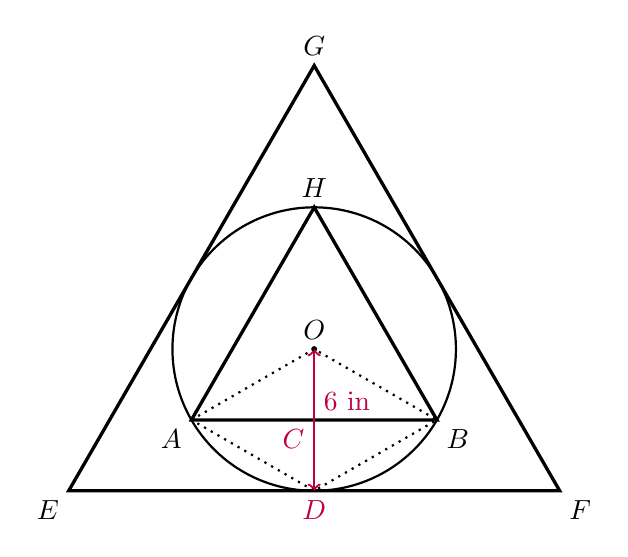
\begin{tikzpicture}[scale=0.3]
		\draw[thick] (0,0) circle [radius=6];
		\draw[very thick] (0,6) -- (-5.19615,-3) -- (5.19615,-3) -- cycle;
		\draw[very thick] (0,12) -- (-10.3923,-6) -- (10.3923,-6) -- cycle;
		
		\draw[fill=black] (0,0) circle [radius=0.1];
		\node[above] at (0,0) {$O$};
		
		\draw[<->][thick][purple] (0,0) -- (0,-6);
		\node[below][purple] at (0,-6) {$D$};
		\node[above right][purple] at (0,-3) {$6$ in};
		\node[below left][purple] at (0,-3) {$C$};
		
		\draw[dotted][thick] (-5.19615,-3) -- (0,0) -- (5.19615,-3) -- (0,-6) -- cycle;
		\node[below left] at (-5.19615,-3) {$A$};
		\node[below right] at (5.19615,-3) {$B$};
		\node[below left] at (-10.3923,-6) {$E$};
		\node[below right] at (10.3923,-6) {$F$};
		\node[above] at (0,12) {$G$};
		\node[above] at (0,6) {$H$};
		\end{tikzpicture}
	\end{center}
	
	% Reasoning
	\paragraph{Reasoning}
	\begin{quotation}
	
	The shortest distance between two parallel lines is the length of the perpendicular segment that connects them. Draw $\overline{OD}$ as a radius of circle $O$ such that $\overline{OD}\bot\overline{AB}$ and $\overline{OD}\bot\overline{EF}$. Since $\overline{OD}$ is a radius perpendicular to chord $AB$, it bisects $\overline{AB}$ (5); therefore $\overline{OD}$ is a perpendicular bisector of $\overline{AB}$. Let the point of intersection between $\overline{AB}$ and $\overline{OD}$ be $C$; since $\overline{OD}$ bisects $\overline{AB}$, $C$ is equidistant from $A$ and $B$; therefore $AC=CB$. Since $\overline{OD}\bot\overline{AB}$, $\angle ACO$, $\angle BCO$, $\angle ACD$, and $\angle BCD$ are right angles and have measures that are equal to 90\textdegree.
	
	Since an equilateral triangle is also equiangular, it is a regular polygon by definition (3). Since the central angle of a regular $n$-gon is $\frac{360\text{\textdegree}}{n}$ (1), and since a triangle has 3 sides, the central angle of an equilateral triangle is $\frac{360\text{\textdegree}}{3}=120$\textdegree; since $\angle AOB$ is a central angle of a regular polygon by definition (4), its measure is 120\textdegree. Since $\overline{OA}$, $\overline{OD}$, and $\overline{OB}$ are radii of circle $O$, they are congruent and are given to be 6 inches long. By the Isosceles Triangle Theorem, $\angle OAB\cong\angle OBA$ and therefore $\text{m}\angle OAB=\text{m}\angle OBA$. By the Triangle Sum Theorem (1), $\text{m}\angle OAB+\text{m}\angle OAB+\text{m}\angle OBA=180$\textdegree; after substitution, $120+\text{m}\angle OAB+\text{m}\angle OBA=180$; after subtracting 120 from both sides, $\text{m}\angle OAB+\text{m}\angle OBA=180-120=60$; thus $\text{m}\angle OAB=\text{m}\angle OBA=\frac{60}{2}=30$. By the Triangle Sum Theorem (1), $\text{m}\angle OAC+\text{m}\angle ACO+\text{m}\angle COA=180$\textdegree and $\text{m}\angle OBC+\text{m}\angle BCO+\text{m}\angle COB=180$\textdegree. After respective substitution, $30+90+\text{m}\angle COA=180$ and $30+90+\text{m}\angle COB=180$; thus $\text{m}\angle COA=180-30-90=60$ and $\text{m}\angle COB=180-30-90=60$. By the 30\textdegree-60\textdegree-90\textdegree \space Triangle Theorem (2), $AO=2CO$ and $BO=2CO$. After dividing both sides by 2, $CO=\frac{AO}{2}$; with $AO=6$, $CO=\frac{6}{2}=3$ by substitution. By the SAP, $CO+CD=OD$; with $OD=6$ and $CO=3$, $3+CD=6$; after subtracting 3 from both sides, $CD=6-3=\boxed{3 \text{  in}}$. Since $\overline{CD}$ is a perpendicular segment that connects parallel sides of the two triangles, its length is the solution to this problem.
	\end{quotation}
	
	\paragraph{External References}
	
	\begin{enumerate}
		\item Textbook Ch. 4, Pg. 223: Triangle Sum Theorem
		\item Textbook Ch. 5, Pg. 358: 30\textdegree-60\textdegree-90\textdegree \space Triangle Theorem
		\item Textbook Ch. 6, Pg. 382: Definition of a Regular Polygon
		\item Textbook Ch. 9, Pg. 601: The Central Angle of a Regular Polygon
		\item Textbook Ch. 11, Pg. 759: Radius $\bot$ to chord $\rightarrow$ radius bisects chord and its arc
	\end{enumerate}

\end{document}